\chapter{Artificial Neural Networks (ANNs)}
\begin{idea}
\begin{itemize}
\item \textbf{Artificial Neural Networks (ANNs):} Computational models inspired by the brain's structure and function.
\item \textbf{Neurons:} Processing units in ANNs that apply weights to inputs and pass through activation functions.
\item \textbf{Activation Functions:} Introduce non-linearity to neuron outputs, enabling complex pattern capturing.
\item \textbf{Loss Function:} Measures the discrepancy between predicted and actual outputs.
\item \textbf{Training:} Process of adjusting weights to minimize the loss function.
\item \textbf{Gradient Descent:} Optimization algorithm that updates weights in the direction of loss reduction.
\item \textbf{Simple Fully Connected Network:} Neurons in one layer connected to all in the next; input passes through hidden layers to produce output.
\item \textbf{Hyperparameters:} Settings chosen prior to training, such as learning rate, batch size, and network architecture.
\item \textbf{Optimizers:} Algorithms that control weight updates during training (e.g., SGD, Adam).
\item \textbf{Normalization:} Techniques like Batch Norm and Layer Norm stabilize training by normalizing input or activation distributions.
\item \textbf{Regularization:} Techniques like Dropout and Weight Decay prevent overfitting by adding constraints or penalties.
\end{itemize}
\end{idea}

\section{Neuron}

\textbf{Simplified Biological Neuron:}
\begin{itemize}
    \item \textbf{Dendrites} recieve information from other neurons
    \item \textbf{Cell body} consolidates information from the dendrites
    \item \textbf{Axon} passes information to other neurons
    \item \textbf{Synapse} is the area where the axon of one neuron and the dendrite of another connect
\end{itemize}

\begin{figure} [h!t]
    \centering
    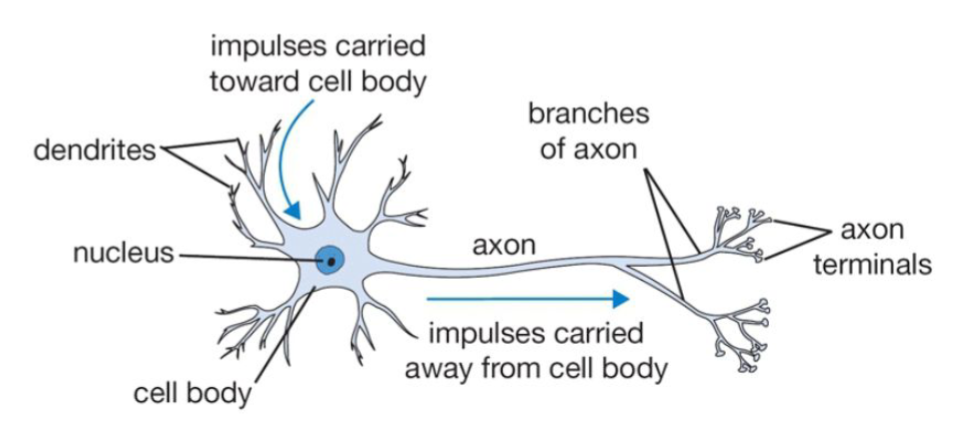
\includegraphics[width=0.5\linewidth]{bioneuron.png}
    \caption{Simplified Biological Neuron}
    \label{fig:enter-label}
\end{figure}

Neurons \textbf{fire} on stimuli: edges, lines, angles, movements, familiar faces, etc. regardless of scale, rotation and translation.\\

\textbf{Artificial Neuron}:

\begin{itemize}
    \item $\mathbf{x}_i$ is the \textbf{input} such as a pixel in an image
    \item $\mathbf{w}_i$ is the \textbf{weight} for input $\mathbf{x}_i$ that we learn for this particular input
    \item $\mathbf{b}$ is the \textbf{bias}, a weight we learn with no input
    \item $\mathbf{f}$ is the \textbf{activation function} that determines how our output changes with the sum of all weight-input products
    \item $\mathbf{y}$ is the\textbf{ output} such as the class an image belongs to
\begin{figure}[h!t]
    \centering
    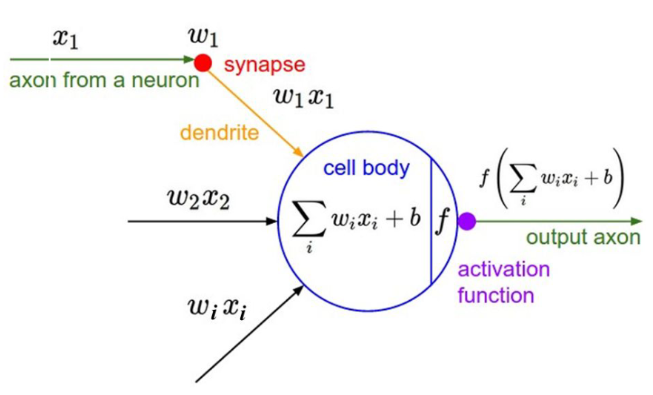
\includegraphics[width=0.5\linewidth]{artificialneuron1.png}
    \caption{Mathematical Representation of Artificial Neuron}
    \label{fig:enter-label}
\end{figure}
    \item Basically, we take the \textbf{weighted sum of all inputs}, \textbf{add the bias term}, then pass the result to the \textbf{activation function}. The result of the activation function is the \textbf{output}.
\[ \Huge y = f(w \cdot x + b) \]

\end{itemize}
\begin{figure} [h!t]
    \centering
    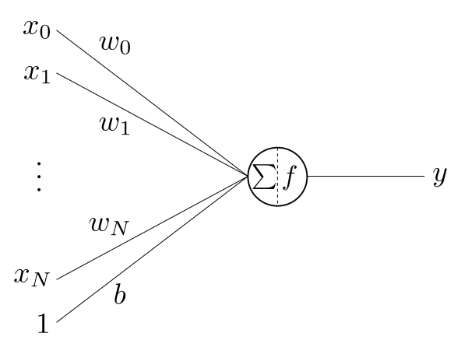
\includegraphics[width=0.5\linewidth]{artificialneuron2.png}
    \caption{Vector Representation of Artificial Neuron}
    \label{fig:enter-label}
\end{figure}
\section{Activation Function}

\textbf{Linear Activation Function}
\begin{definition}
    \textbf{Linear Activation Function}: a mathematical function that produces an \textbf{output directly proportional to its input}. In other words, for any given input, the output increases or decreases at a constant rate without any bending or non-linear behavior.
\end{definition}
\begin{figure}[h!t]
    \centering
    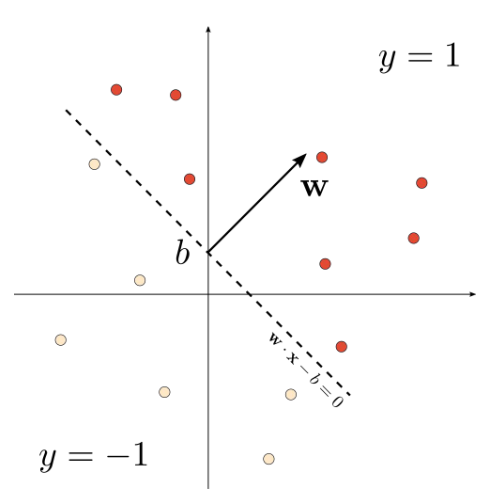
\includegraphics[width=0.4\linewidth]{linearactivation.png}
    \caption{Linear Activation Function}
    \label{fig:enter-label}
\end{figure}
\begin{itemize}
    \item When the activation function is a simple linear function:
\[ y = f(w \cdot x + b) \longrightarrow y = w \cdot x + b\]
    \item This is a special equation and becomes more clear if we write it out for 2D:
\[y = w_0 x_0 + w_1 x_1 + b\]
    \item Recall general equation of line:

\[Ax + By - C = 0\]

    \item The bias is related to the offset of the line from the origin and allows us to create a boundary between data that doesn't have to go through the origin
\begin{definition}
   \textbf{ Bias Term:} a \textbf{constant} value that's added to the weighted sum of inputs in a neuron or model, allowing the neuron to \textbf{shift the activation function's output} up or down, effectively \textbf{adjusting the decision boundary} of the neuron's response. The bias term is \textbf{learnable} during the training process, just like the weights associated with the inputs
\end{definition}
    \item \(y = w \cdot x + b\)  is a generalized line for any dimension, known as \textbf{hyperplane}, splitting the n-dimensional input space into 2 parts
    \item Linear activation functions are \textbf{not usually practical} since most real datasets are not linearly separable (we can't usually find a straight line that separates classes well in a classification problem)
    \item We can learn \textbf{non-linear transformations} of our data to help
\begin{figure}[h!t]
        \centering
        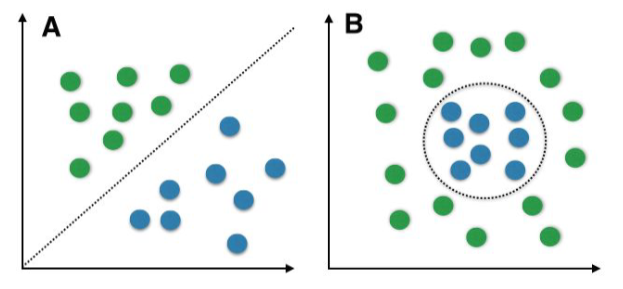
\includegraphics[width=0.5\linewidth]{linearvsnonlinearAF.png}
        \caption{Most datasets are not linearly separable like A}
        \label{fig:enter-label}
    \end{figure}
    \item Multiple layers with non-linear transformations are useful, while \textbf{there is no advantage from multiple linear layers}, since the composite is a linear layer and reduces the network's ability to capture complex patterns in data
\end{itemize}
\textbf{Perceptrons (Binary Activation Function)}
\begin{definition}
   \textbf{ Perceptron Activation Function:} a decision rule that outputs \textbf{1 when the weighted sum of inputs exceeds a threshold, and outputs 0 otherwise}. This decision guides the activation of a perceptron in a basic neural network unit.
\end{definition}
\begin{figure}[h!t]
    \centering
    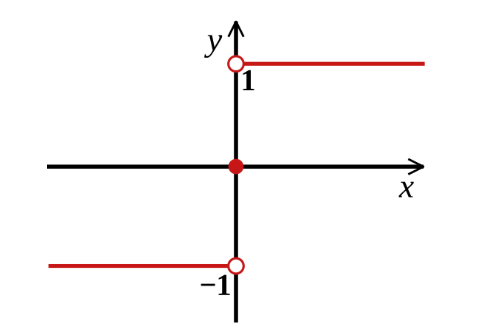
\includegraphics[width=0.4\linewidth]{perceptrons.png}
    \caption{Perceptrons}
    \label{fig:enter-label}
\end{figure}
\begin{itemize}
\item The first artificial neurons (1943-1970s) use a simple binary activation function based on which side of the hyperplane the input is
\item Examples of these functions include the \textbf{Sign function} and the \textbf{Heaviside (unit) step function}
\[f(x) = sign(x)\]
\[f(x) = \begin{cases}
        0, & \text{if } x < 0, \\
        1, & \text{if } x \geq 0.
      \end{cases}\]
      \item The \textbf{decision boundary} is the hyperplane, or the \textbf{threshold that separates the classes} in the binary classification problem. 
      \item These functions are \textbf{not differentiable, contiuous or smooth}


\end{itemize}
\textbf{Sigmoid Activation Function}
\begin{figure}[h!t]
    \centering
    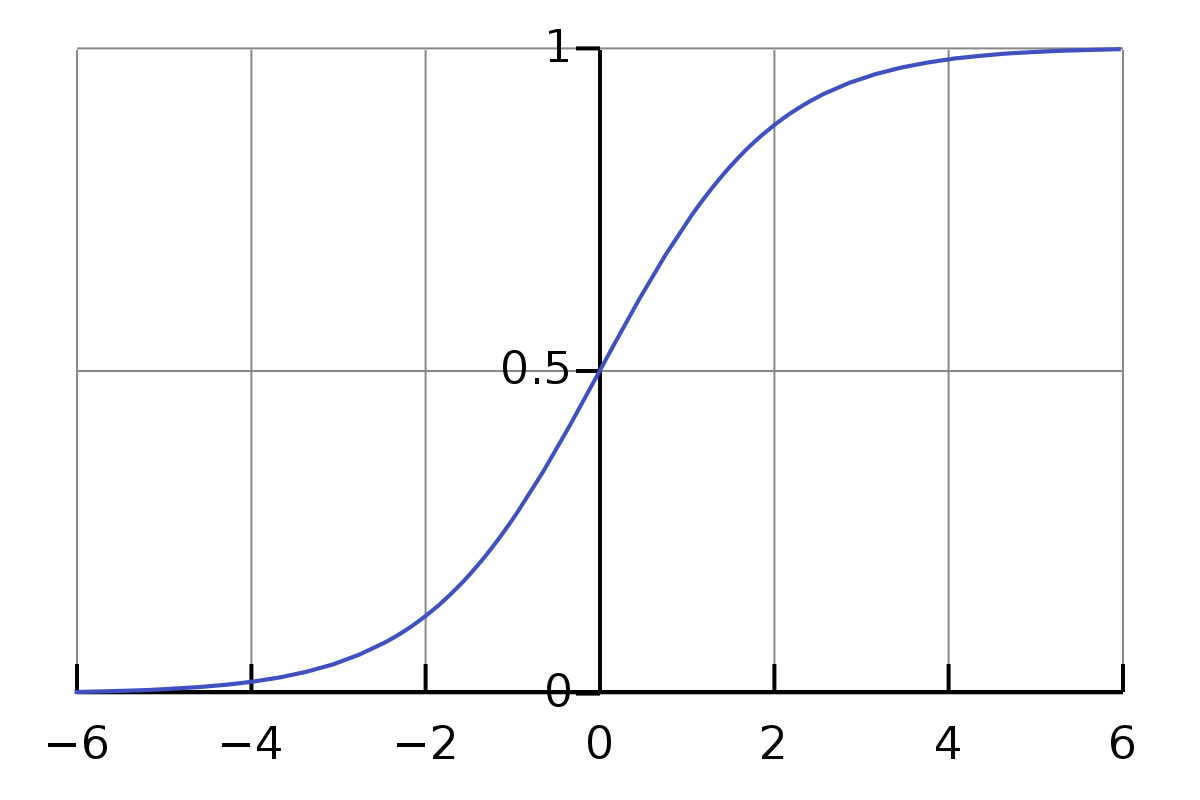
\includegraphics[width=0.5\linewidth]{sigmoid.png}
    \caption{Sigmoid Function}
    \label{fig:enter-label}
\end{figure}
\begin{definition}
    \textbf{Sigmoid Activation Function:} a mathematical function that \textbf{smoothly} maps input values to a specified output range. It is characterized by an S-shaped curve and is commonly used in neural networks to \textbf{introduce non-linearity}, allowing the network to capture complex relationships in data. The sigmoid function is particularly useful for transforming raw scores into probabilities or for controlling the strength of neuron activations.
\end{definition}
\begin{itemize}
    \item Sigmoid activation functions were most common before 2012
    \item \textbf{Easily differentiable, smooth, continuous}
    \item Range between [-1, 1] or [0, 1]
    \item There are many sigmoid functions, the most common are \textbf{Hyperbolic tangent} and \textbf{Logistic functions}:

\[f(x) = \text{tanh}(x)\]

\[f(x) = \frac{1}{1 + e^{-x}}\]
\item Saturated neurons "kill" the gradients
\begin{definition}
    \textbf{Gradients:} represent the directions and magnitudes by which the network's internal settings (weights and biases) should be adjusted to minimize the difference between its predictions and the actual target values. Gradients guide the network during training, helping it learn how to make better predictions by fine-tuning its parameters based on the errors it makes.
\end{definition}
\item Gradients become vanishingly small very quickly away from x = 0
\begin{theorem}
    \textbf{Vanishing Gradient Problem:}  pertains to the phenomenon wherein the \textbf{gradients of the loss function} with respect to the parameters of the earlier layers \textbf{become extremely small} as they are back-propagated through the network during the learning process. This reduction in gradient magnitude \textbf{diminishes the weight updates applied to the earlier layers} during optimization, causing these layers to \textbf{learn at a significantly slower rate or even stagnate} in terms of learning progress. As a consequence, the \textbf{network struggles to capture complex relationships} in the data, hindering its ability to generalize and make accurate predictions.
\end{theorem}
\end{itemize}
\begin{figure}[h!t]
    \centering
    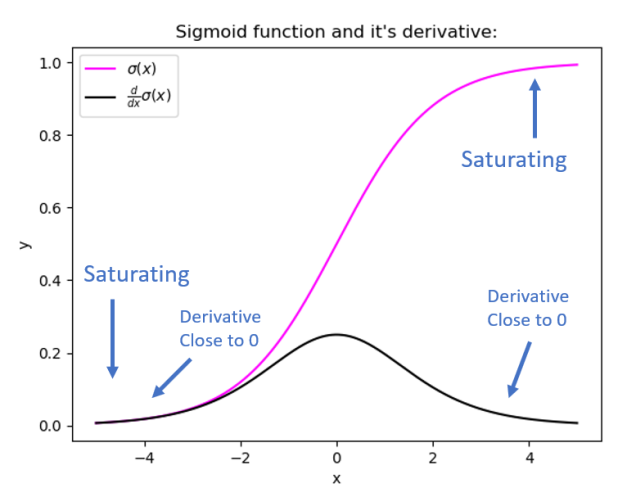
\includegraphics[width=0.5\linewidth]{vanishinggradientproblem.png}
    \caption{Vanishing Gradient Problem}
    \label{fig:enter-label}
\end{figure}

\newpage

\textbf{ReLU Activation Function}

\begin{definition}
\textbf{ ReLU Activation Function:} turns \textbf{on for positive input values}, allowing signals to pass unchanged. For \textbf{negative inputs, it outputs zero}, which helps the network introduce non-linearity and learn complex patterns in data. ReLU helps with the vanishing gradient problem, though variations like Leaky ReLU address potential issues of inactive neurons during training.
\end{definition}

\begin{figure}[h!t]
    \centering
    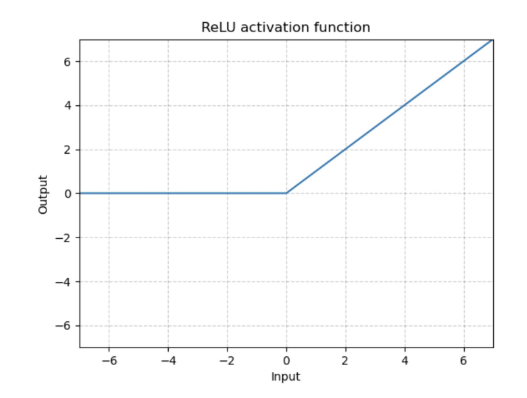
\includegraphics[width=0.5\linewidth]{ReLU.png}
    \caption{ReLU Activation Function}
    \label{fig:enter-label}
\end{figure}

\begin{itemize}
    \item Modern deep learning typically uses the \textbf{Rectified Linear Unit (ReLU)} based activation functions:
    \begin{itemize}
        \item \textbf{ReLU}:

\[\text{ReLU}(x) = (x)^+ = \max(0, x)\]

        \item \textbf{Leaky ReLU}:

\[
\text{LeakyReLU}(x) = \begin{cases}
x, & \text{if } x \geq 0 \\
\text{negative\_slope} \cdot x, & \text{otherwise}
\end{cases}\]


        \item \textbf{Parametric ReLU:}

\[\text{PReLU}(x) = \begin{cases}
x, & \text{if } x \geq 0 \\
a \cdot x, & \text{otherwise}
\end{cases}\]
\item These functions have very \textbf{easy derivaties}: 0 or 1; use 0 at x = 0
\end{itemize}
\item We can also approximate ReLU activation by \textbf{continuous functions}:
\begin{itemize}
    \item \textbf{SiLU (Swish)}:

\[\text{SiLU}(x) = x \cdot \sigma(x) = \frac{x}{1 + e^{-x}}\]

    \item \textbf{SoftPlus}:


\[\text{SoftPlus}(x) = \frac{1}{\beta} \cdot \log(1 + e^{\beta x})\]

    \item These work \textbf{on par or better} than ReLU functions  due to mitigating issues like the \textbf{vanishing gradient problem}, dead neurons, lack of smoothness, and noise sensitivity that can arise with the original ReLU function. These approximations offer improved stability, controlled activation behavior, and better optimization dynamics for specific tasks and network architectures.

\end{itemize}
\end{itemize}

\section{Training Neural Networks}

How do we learn the\textbf{ weights} and\textbf{ bias }of a neural network?\\
Input: \( x \), Predicted Output: \( y \), Ground Truth Label: \( t \), Neuron \( M(w;x) \)
\begin{enumerate}
  \item \textbf{Prediction:} Make a prediction for some input data \( x \), with a known correct output \( t \):
  \[ y = M(w;x) \]
  
  \item \textbf{Comparison:} Compare the correct output with our predicted output to compute loss:
  \[ E = \text{Loss}(y, t) \]
  
  \item \textbf{Adjustment:} Adjust the weights/bias to make the prediction closer to the ground truth, i.e., minimize error.
  \item \textbf{Repetiton:} Repeat until we have an acceptable level of error.

\end{enumerate}
This process gradually improves a network's ability to solve a problem.

\begin{definition}
    \textbf{Forward Pass:} input data is fed into a neural network, and it \textbf{flows through the layers}, undergoing computations using the network's parameters (weights and biases). This process generates predictions or output values based on the input data. Used for both \textbf{training and inference}.
\end{definition}

\begin{definition}
    \textbf{Backward Pass:} also known as \textbf{backpropagation}, this step follows the forward pass. It involves \textbf{calculating the gradients of the loss function} with respect to the network's parameters. These gradients indicate how much each parameter needs to be \textbf{adjusted} to reduce prediction errors. The gradients are then used to update the parameters using optimization algorithms. Used only for \textbf{training}.
\end{definition}

The forward pass is the initial step that \textbf{produces predictions} based on input data. The backward pass is crucial for \textbf{training} the network. By computing gradients during the backward pass, the network's parameters are adjusted in a way that \textbf{reduces prediction errors}. This adjustment is \textbf{iteratively repeated} through multiple forward and backward passes, refining the network's parameters to make better predictions over time.\\
\\In summary, the \textbf{forward pass generates predictions}, while the \textbf{backward pass calculates gradients to fine-tune the network's parameters}, enabling it to learn and improve its performance.

\begin{idea}
    All activation functions used in modern neural networks trained with backpropogation are both differentiable and non-linear.
\end{idea}

\section{Loss Function}
\begin{definition}
    \textbf{Loss Function:} computes \textbf{how bad predictions are} compared to the ground truth labels. Large loss means the network's predictions differ from the ground truth. Small loss means the network's prediction matches the ground truth.
\end{definition}

We want to calculate the error over \textbf{all training samples} (to get the average error).

\begin{figure}[h!t]
    \centering
    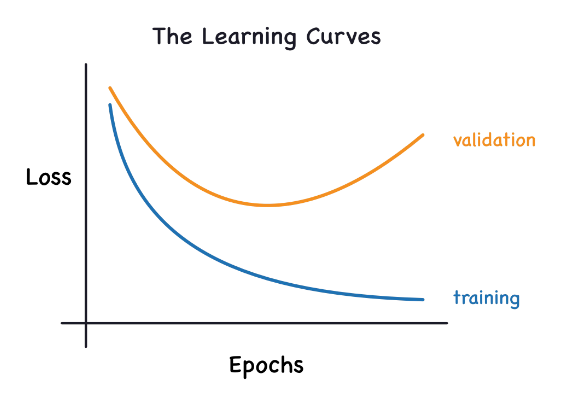
\includegraphics[width=0.25\linewidth]{lossfunction.png}
    \caption{Learning Curves}
    \label{fig:enter-label}
\end{figure}

\newpage

\begin{example}
    Suppose we want to train a linear neuron to differentiate images into three classes:
\end{example}
\begin{figure}[h!t]
    \centering
    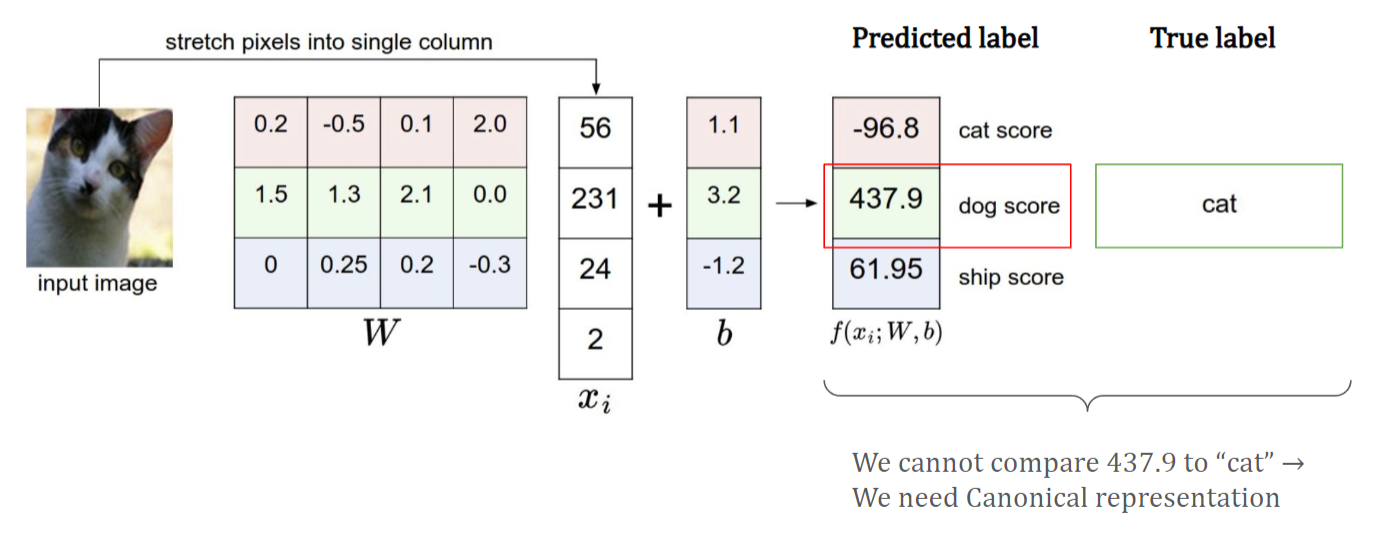
\includegraphics[width=0.75\linewidth]{whysoftmax.png}
    \caption{Why we need Softmax}
    \label{fig:enter-label}
\end{figure}
We need a way that will allow us to \textbf{represent the output} in a way that can be \textbf{compared to the true label} so that we may see if the model's predictions are accurate or not. Enter: \textbf{Softmax}.

\begin{definition}
    \textbf{Softmax function:} \textbf{normalizes the logits} into a categorical probability distribution over all possible classes. Produces normalized probabilites for multiple classes.
\end{definition}

\begin{figure}[h!t]
    \centering
    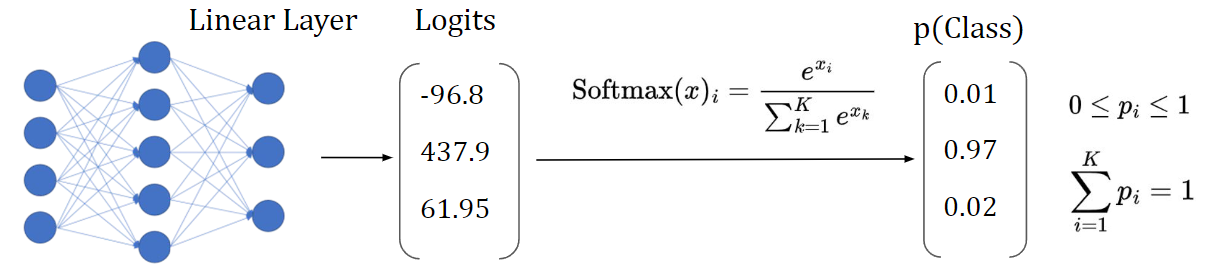
\includegraphics[width=0.75\linewidth]{softmax.png}
    \caption{Softmax Function}
    \label{fig:enter-label}
\end{figure}
We still need to map "cat" to a \textbf{vector} so that it can be compared with the softmax output. A way to map categories to vector representation is \textbf{One-hot encoding}.

\begin{definition}
    \textbf{One-hot encoding:}  a \textbf{binary representation} technique used to convert categorical variables into a \textbf{numerical format}. Each category is represented as a binary vector where a single element is set to \textbf{1} (indicating the \textbf{presence} of that category) while all other elements are set to \textbf{0} (indicating the \textbf{absence} of other categories).
\end{definition}
\begin{figure}[h!t]
    \centering
    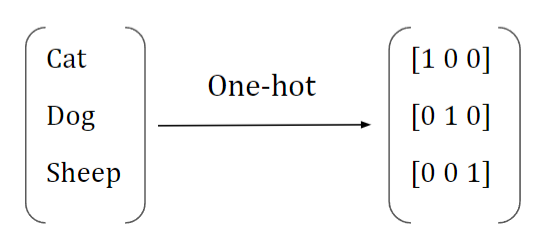
\includegraphics[width=0.25\linewidth]{onehotencoding.png}
    \caption{One-hot encoding}
    \label{fig:enter-label}
\end{figure}
Now that the output of the model and the classes have been converted to comparable forms, how do we determine the accuracy of the model? We use \textbf{Loss functions}:
\begin{enumerate}
    \item \textbf{Mean Squared Error (MSE)}: mostly used for \textbf{regression} problems (predicting continuous numeric output)
\[
MSE = \frac{1}{N} \sum_{n=1}^{N} (y_{\text{predicted}, i} - y_{\text{actual}, i})^2
\]

Where:
\begin{align*}
n &: \text{Number of data points (training samples)} \\
y_{\text{predicted}, i} &: \text{Predicted value for the } i\text{th data point} \\
y_{\text{actual}, i} &: \text{Actual target value for the } i\text{th data point}
\end{align*}
\begin{figure}[h!t]
    \centering
    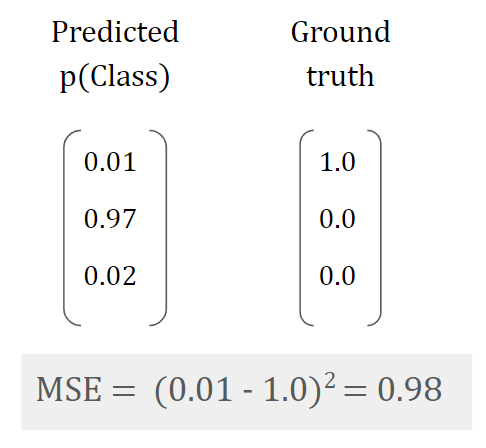
\includegraphics[width=0.25\linewidth]{mse.png}
    \caption{Mean Squared Error}
    \label{fig:enter-label}
\end{figure}
    \item \textbf{Cross Entropy (CE)}: mostly used for \textbf{multi-class classification} problems
\[
CE = - \frac{1}{N} \sum_{n=1}^{N} \sum_{k=1}^{K}  y_{\text{actual}, n, k} \cdot \log(y_{\text{predicted}, n, k}) 
\]

Where:
\begin{align*}
N &: \text{Number of data points (training samples)} \\
K &: \text{Number of classes} \\
y_{\text{actual}, n, k} &: \text{Actual target value (1 or 0) for the } n\text{th data point and } k\text{th class} \\
y_{\text{predicted}, n, k} &: \text{Predicted probability for the } k\text{th data point belonging to the } k\text{th class} \\
\end{align*}
\begin{figure}[h!t]
    \centering
    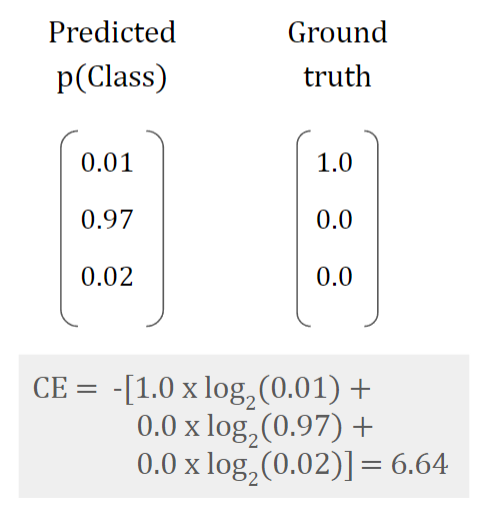
\includegraphics[width=0.25\linewidth]{ce.png}
    \caption{Cross Entropy Error}
    \label{fig:enter-label}
\end{figure}

    \item \textbf{Binary Cross Entropy (BCE)}: mostly used for \textbf{binary classification} problems
\[
BCE = -\frac{1}{N} \sum_{n=1}^{N} \left( y_{\text{actual}, n} \cdot \log(y_{\text{predicted}, n}) + (1 - y_{\text{actual}, n}) \cdot \log(1 - y_{\text{predicted}, n}) \right)
\]

Where:
\begin{align*}
N &: \text{Number of data points} \\
y_{\text{actual}, n} &: \text{Actual target value (0 or 1) for the } n\text{th data point} \\
y_{\text{predicted}, n} &: \text{Predicted probability for the } n\text{th data point} \\
\end{align*}
\end{enumerate}

\section{Gradient Descent}
\begin{definition}
    \textbf{Gradient Descent:} an optimization algorithm used in machine learning to \textbf{iteratively} adjust the parameters of a model in the \textbf{direction that decreases the model's error}, guided by the \textbf{gradient} of the error with respect to those parameters.
\end{definition}

A neural network layer with two neurons: 
\[y_1 = f(w_1 \cdot x + b_1)\]
\[y_2 = f(w_2 \cdot x + b_2)\]
can represent a neural network easier with a \textbf{matrix} where each neuron's weight vector is a \textbf{row of the weight matrix W} and the input is a \textbf{column vector x}:
\[y=f(Wx+b)\]
This is relevant for debugging the dimensions of tensors.

\begin{figure}[h!t]
    \centering
    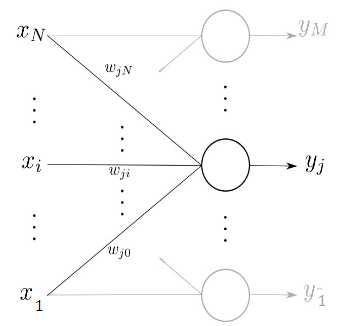
\includegraphics[width=0.3\linewidth]{twoneurons.png}
    \caption{NN layer represented by vectors}
    \label{fig:enter-label}
\end{figure}
In order to improve our network, we want to know how to change each of our neuron's weights \(w_ji\) to \textbf{reduce error} \(E\). Basically, we want to find the weights that are \textbf{increasing the error} and change them in the \textbf{opposite direction} of the current function to \textbf{correct} them. To do this, we will use \textbf{Gradient Descent}.

\begin{idea}
    In the context of this course, \textbf{gradients and derivatives are the same thing}. The \textbf{vector} of partial derivatives for all weights is the \textbf{gradient}. The \textbf{direction} of the gradient is the \textbf{direction the function is increasing}. The \textbf{magnitude} of the gradient is the \textbf{rate of increase}.
\end{idea}

First, we need to know how our error changes with \textbf{each individual weight}:
\[\frac{\partial E}{\partial w_{ji}}\]
This is relatively simple to calculate adjacent to the output layer. Adjusting weights according to the slope (gradient) will guide us to the minimum (or maximum) error. We do this by computing the \textbf{gradient of loss with respect to each weight}. That will tell us the direction in which the weight is increasing the loss.


\begin{figure}[h!t]
    \centering
    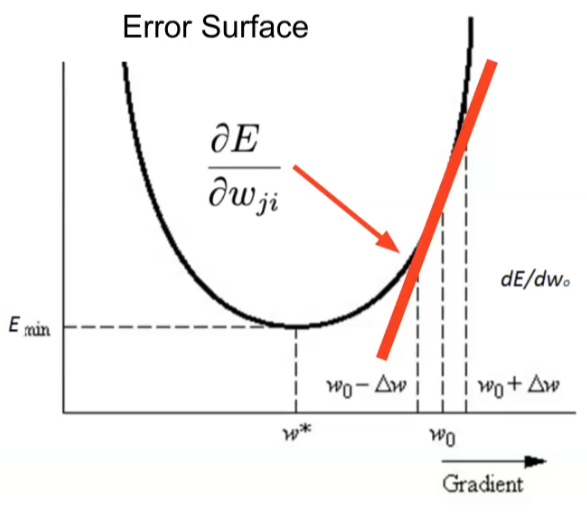
\includegraphics[width=0.5\linewidth]{gradientdescent.png}
    \caption{Gradient Descent. The graph represents the Error (loss) function and the red tangent line is gradient of loss.}
    \label{fig:enter-label}
\end{figure}


\[ \text{\textbf{Gradient Descent Formula:}    } w_{ji}^{t+1} = w_{ji}^{t} - \eta \frac{\partial E}{\partial w_{ji}}\]


\[\Delta w_{ji} = \eta \frac{\partial E}{\partial w_{ji}}\]


Where \(\eta\) is the learning rate (step size).\\

\begin{idea}
    A \textbf{positive} gradient at a weight means that the weight is\textbf{ contributing} to the loss. This is why we negate it in the Gradient Descent Formula
\end{idea}

\begin{example}
\textbf{Delta Rule} for Single Weight/Training Example


\[E = (y - t)^2  \text{  and  } f(x) = \frac{1}{1+e^{-x}}\]
To solve this, we need to use the \textbf{Chain Rule}:


\[ \frac{dE}{dw_p} = (\frac{dE}{dy}) (\frac{dy}{da}) (\frac{da}{dw_p}) \]
\begin{itemize}
    \item \(a = \sum_{p} w_p x_p + b\)    (summation of inputs)
    \item \(y = f(a)\)
    \item \(\frac{dE}{dw_p} \text{ represents the derivative of the error } E \text{ with respect to the weight } w_p.\)
    \item \(\frac{dE}{dy} \text{ represents the derivative of the error } E \text{ with respect to the output } y.\)
    \item \(\frac{dy}{da} \text{ represents the derivative of the output } y \text{ with respect to the input } a.\)
    \item \(\frac{da}{dw_p} \text{ represents the derivative of the input } a \text{ with respect to the weight } w_p.\)\\
\end{itemize}

Let's calculate each of these derivatives:


\[\frac{dE}{dy} = (\frac{d(y-t)^2}{dy}) = 2(y-t)\]


\[\frac{dy}{da} = (\frac{d{\frac{1}{1+e^{-a}}}}{da}) = (1-y)(y) \text{   (useful property of sigmoid functions)}\]

\[\frac{da}{dw_p} = x_p\]


\[\frac{dE}{dw_p} = 2(x_p)((y-t)((1-y)(y)))\]
\end{example}

\begin{figure}[h!t]
    \centering
    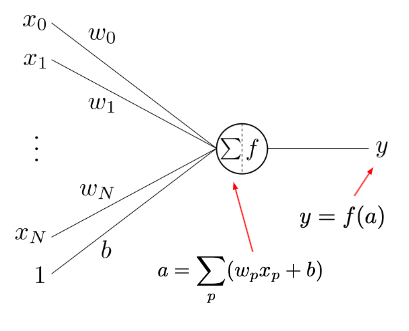
\includegraphics[width=0.4\linewidth]{deltaruleexample.png}
    \caption{Delta Rule Example}
    \label{fig:enter-label}
\end{figure}

\newpage

\section{Neural Network Architectures}

\textbf{XOR Problem}\\

\begin{figure} [h!t]
    \centering
    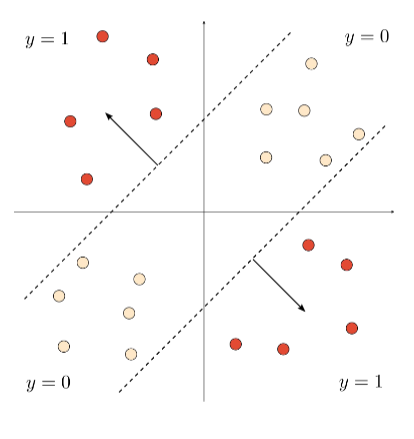
\includegraphics[width=0.35\linewidth]{xor.png}
    \caption{XOR Function}
    \label{fig:enter-label}
\end{figure}

Having a single decision boundary (a single NN layer) is not enough to solve many problems. The most famous such problem is the \textbf{XOR function}, which \textbf{needs two decision boundaries} to solve (more than one line).

\begin{definition}
    \textbf{XOR Function:} short for "exclusive OR," is a logical operation that takes in two inputs and produces an output. The output is \textbf{true (or 1) when the inputs are different from each other}, and \textbf{false (or 0) when the inputs are the same}. In other words, if one input is true and the other is false, the XOR function gives a true output. If both inputs are the same (both true or both false), the XOR function gives a false output.
\end{definition}

We solve this by having \textbf{at least one hidden neural network layer}. In fact in the limit of an infinitely-wide neural network with at least one hidden layer, \textbf{NN is a universal function approximator}. This means that if this hidden layer is made extremely wide (with many neurons), and there's at least one hidden layer, the neural network becomes capable of \textbf{approximating almost any kind of function}.


\begin{definition}
   \textbf{ Hidden Layer:} a set of neurons that process information \textbf{between the input and output layers}, capturing complex patterns in the data. It's called "hidden" because it's \textbf{not directly connected to the input or output} of the network.
\end{definition}

\noindent\textbf{Credit Assignment Problem}\\
\begin{figure}[h!t]
    \centering
    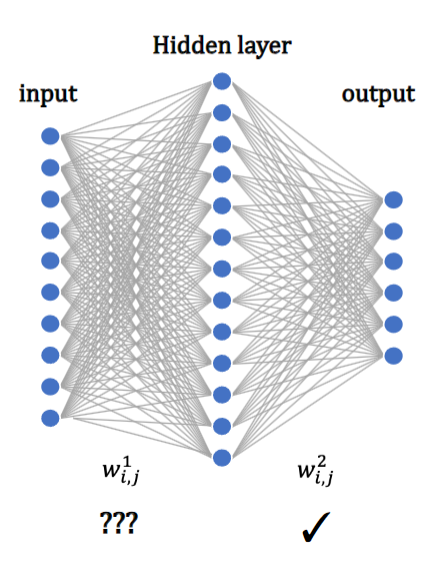
\includegraphics[width=0.3\linewidth]{creditassignment.png}
    \caption{Backpropogation}
    \label{fig:enter-label}
\end{figure}
Neural networks up until the 1970s were not very useful for two main reasons:
\begin{enumerate}
    \item Not clear how to train a NN of more than 1 layer (known as the \textbf{credit assignment problem})
    \item A neural network of only \textbf{one layer cannot describe complex functions}, two or more can represent any function (in theory with infinite width).
\end{enumerate}
\begin{definition}
    \textbf{Credit Assignment Problem:} the challenge of figuring out \textbf{how much each neuron in a network contributed to the final prediction or output}. It's about understanding which parts of the network were most \textbf{responsible for the outcome} and how changes in \textbf{individual neurons affect the overall performance}. 
\end{definition}

\begin{idea}
    Solving the credit assignment problem is essential for training neural networks effectively, as it allows us to identify which parts of the network \textbf{need adjustment or improvement}. Without a clear understanding of credit assignment, it's challenging to fine-tune networks, diagnose issues, and ensure consistent learning and performance improvement.
\end{idea}

The credit assignment problem was solved by \textbf{backpropagation}, a method that describes how to distribute errors to neurons \textbf{not adjacent to the output layer}.

\begin{definition}
    \textbf{Backpropagation}: a method in training neural networks, where the \textbf{network adjusts its internal parameters (weights and biases) by computing the gradient of the loss function} with respect to these parameters. This allows the network to learn and improve its predictions over time.
\end{definition}

Backpropagation uses a \textbf{dynamic programming}-like approach to calculate gradients and adjust weights in neural networks. The combination of \textbf{gradient descent} and \textbf{dynamic programming} is called backpropogation. It propagates error information \textbf{backward} through the layers, updating the weights in a way that \textbf{optimizes the network's performance over time.}  \\

\noindent\textbf{Multiple Layers with Non-Linearity}

\begin{figure}[h!t]
    \centering
    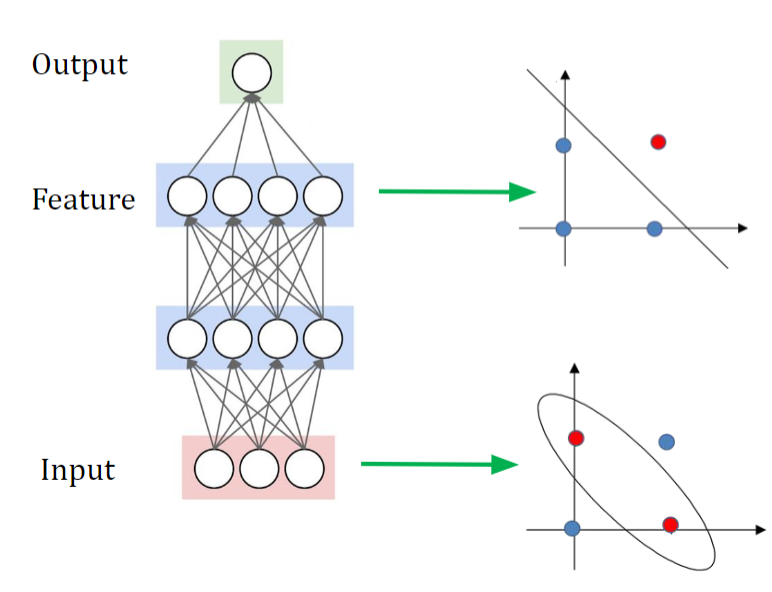
\includegraphics[width=0.4\linewidth]{multiplelayersnonlinearity.png}
    \caption{Multiple Layers with Non-Linearity}
    \label{fig:enter-label}
\end{figure}
\begin{itemize}
    \item Neural networks can be viewed as a way of learning features directly and end-to-end from raw input data.
    \item You can use the activations of the layer before the last layer as high-level features representing the input data.
    \item The goal being that the final layer is presented with a \textbf{linear separation}.
\end{itemize}

\begin{idea}
 Essentially, the network \textbf{maps (or projects) input, which is not linearly separable, to other dimensions (spaces) where it does become linearly separable}. The output layer is a linear layer because by the time the data reaches it, \textbf{it is already linearly separable}. In these hidden layers, the network learns features in the input data.
\end{idea}

\noindent\textbf{Neural Network Architecture}\\
An architecture of a neural network describes the neurons and their connectivity. Architecture selection will greatly affect model performance. It is an example of a very significant \textbf{inductive bias}.
\begin{definition}
\textbf{Feed-Forward Network:} information only flows forward from \textbf{one layer to a later layer}, from the input to the output \textbf{without any loops or cycles}. It's designed to make predictions or classifications based on the input data \textbf{without internal feedback connections}.
\end{definition}
\begin{definition}
\textbf{Fully-Connected Network:} neurons between adjacent layers are \textbf{fully connected}. Each neuron in a given layer is connected to every neuron in the subsequent layer. This creates a \textbf{dense} and \textbf{interconnected structure} that enables \textbf{information to flow freely} between all layers.
\end{definition}
\begin{definition}
\textbf{Number of Layers:} number of \textbf{hidden layers + output layer} (not including input "layer")
\end{definition}

\begin{figure}[h!t]
    \centering
    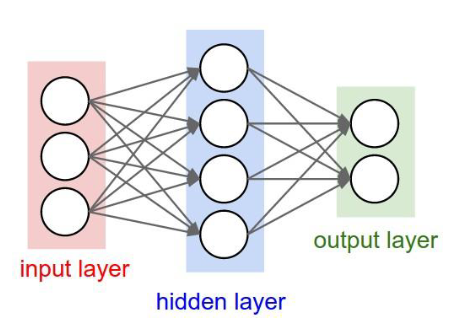
\includegraphics[width=0.3\linewidth]{twolayerNN.png}
    \caption{2-Layer Neural Network}
    \label{fig:enter-label}
\end{figure}
\begin{figure}[h!t]
    \centering
    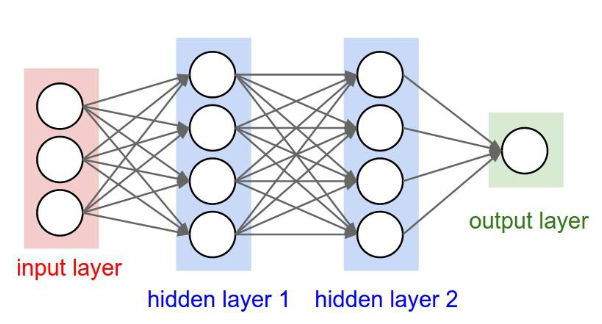
\includegraphics[width=0.325\linewidth]{threelayerNN.png}
    \caption{3-Layer Neural Network}
    \label{fig:enter-label}
\end{figure}

\begin{example}
    Given the code below, for a binary neural network classifier, answer the following questions.
    \begin{verbatim}
 def __init__ ( self ) :
     super ( MLP , self ) . __init__ ()
     self . firstLayer = nn . Linear (20 , 10)
     self . middleLayer = nn . Linear (10 , 10)
     self . lastLayer = nn . Linear (10 , 1)
 def forward ( self , input ) :
     activation1 = self . firstLayer ( input )
     activation1 = F . relu ( activation1 )
     activation2 = self . middleLayer ( activation1 )
     activation2 = F . relu ( activation2 )
     activation3 = self . middleLayer ( activation2 )
     activation3 = F . relu ( activation3 )
     activation4 = self . lastLayer ( activation3 )
     return activation4
    \end{verbatim}
\textbf{What is the input size of the network?:}
\\(20, B) Where B is the batch size.\\
\\\textbf{How many layers are there in the following network?:}
\\There are 4 layers in the network. Recall that the output layer is also considered a layer, while the input layer is not considered.\\
\textbf{\\What is the total number of parameters in the network (including biases)?:}
\\441 = (20*10 + 10) + (10*10 + 10) + (10*10 + 10) + (10*1 + 1)
\end{example}

\begin{idea}
    To calculate the \textbf{number of parameters} for a fully-connected network layer:
\[\text{Number of weights} = \text{Input size (entering layer) } \cdot \text{ Number of Neurons (in layer) } + \text{ Bias Term (for each neuron in layer)}\]
Only include bias term if it is assumed to exist.

\end{idea}

\begin{example}
    Calculating number of parameters (weights) for Fully-Connected Networks:
    \begin{itemize}
        \item Input: 200 x 200 pixels = 40000
        \item 1st hidden layer: 500 neurons
        \item 2nd hidden layer: 200 neurons
    \end{itemize}
(Weights = 40 000 x 500 + 500 x 200) + (Bias = 500 + 200) = 20100700 parameters
\end{example}

\begin{example}
    Calculating number of parameters (weights) for Fully-Connected Networks:
    \begin{itemize}
        \item self.fc1 = nn.Linear(16, 100)
        \item self.fc2 = nn.Linear(32, 100)
    \end{itemize}
(Weights = 16 x 100 + 32 x 100) + (Bias = 100 + 100) = 5000 parameters
\end{example}

\section{Hyperparameters}

While neural network \textbf{parameters}, such as weights, are updated through \textbf{Gradient Descent} \textbf{(Inner loop of optimization)}, \textbf{hyperparameters} are tuned by methods such as \textbf{Grid Search} and\textbf{ Random Search} \textbf{(Outer loop of optimization)}. Most of the time, \textbf{Random Search is all we need} as \textbf{Grid Search is very time consuming and costly}. 

\begin{figure}[h!t]
    \centering
    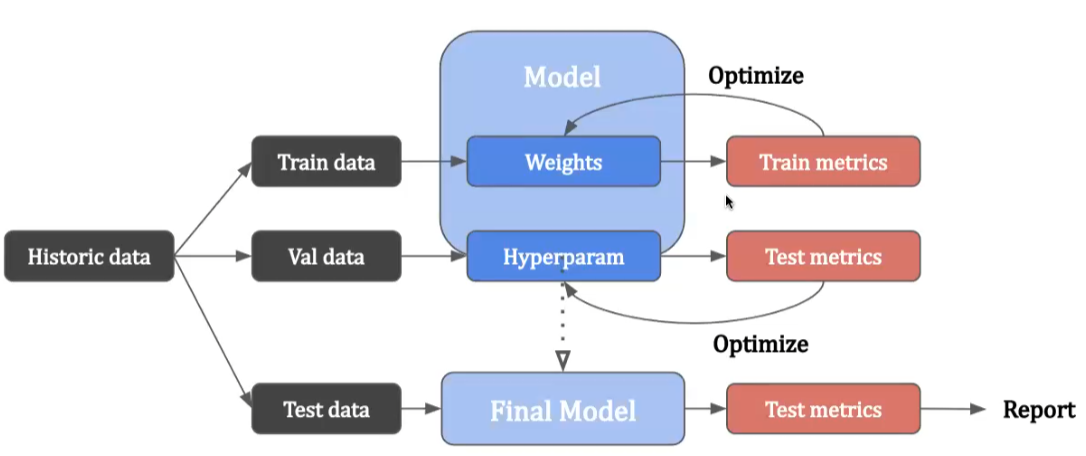
\includegraphics[width=0.75\linewidth]{hyperparams.png}
    \caption{How split data affects optimization}
    \label{fig:enter-label}
\end{figure}

\begin{figure} [h!t]
    \centering
    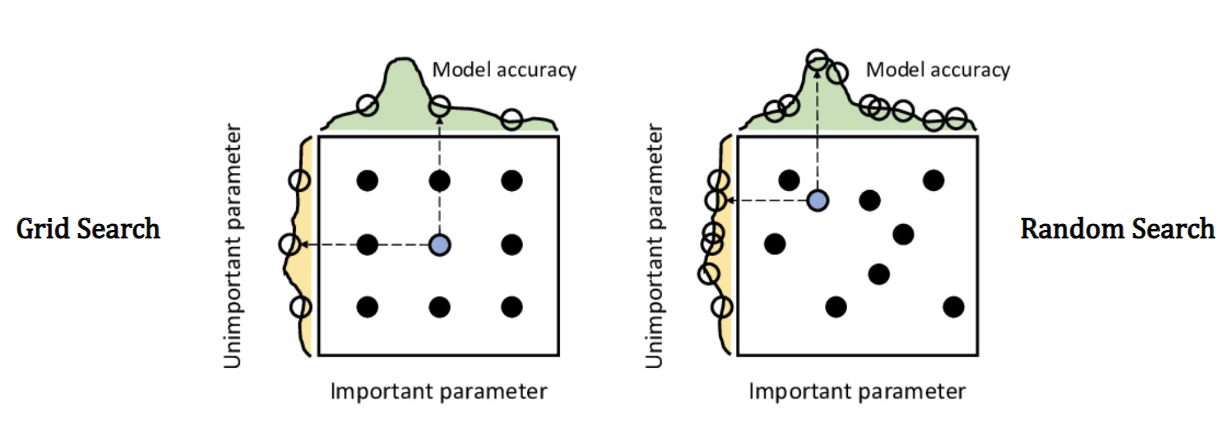
\includegraphics[width=0.75\linewidth]{tuninghyperparams.png}
    \caption{Grid Search and Random Search}
    \label{fig:enter-label}
\end{figure}

\begin{definition}
    \textbf{Grid Search:} involves creating a \textbf{predefined} grid of hyperparameter values to explore. It \textbf{exhaustively evaluates all possible combinations} of these values. It systematically searches through the entire parameter space, testing each combination to find the \textbf{best-performing set} of hyperparameters. Grid search is ideal when the hyperparameter space is relatively small and the interactions between hyperparameters are not too complex.
\end{definition}

\textbf{Pros of Grid Search}:

\begin{itemize}
    \item Exhaustive search that \textbf{guarantees optimal hyperparameters} within the specified search space.
    \item Systematic approach that \textbf{covers all combinations}.
\end{itemize}

\textbf{Cons of Grid Search}:

\begin{itemize}
    \item \textbf{Computationally expensive} when the search space is large.
    \item Inefficient when many \textbf{hyperparameters are not influential}.
\end{itemize}

\begin{definition}
    \textbf{Random Search:} \textbf{randomly} samples hyperparameters from a specified distribution or range. It performs a \textbf{certain number of random trials}, independently of each other, and evaluates the model's performance with each set of hyperparameters. Random search is particularly useful when the search space is large or when the impact of individual hyperparameters is less clear.\textbf{ Generally better than Grid Search}.
\end{definition}

\textbf{Pros of Random Search:}

\begin{itemize}
    \item More \textbf{efficient} when the search space is large or when some hyperparameters are less influential.
    \item \textbf{Less computationally demanding} compared to grid search for large search spaces.
\end{itemize}

\textbf{Cons of Random Search:}

\begin{itemize}
    \item There's no guarantee of finding the optimal hyperparameters, as it \textbf{relies on chance}.
    \item It might require more trials to converge to the best solution compared to grid search.
\end{itemize}

\section{Optimizers}

Defining a loss function turns a \textbf{learning problem into an optimization problem}. An optimizer determines, based on the value of the loss function, \textbf{how each parameter (weight) should change}. The optimizer solves the \textbf{credit assignment problem}. We assign credit to the parameters based on how the network performs by using optimizers that are based on \textbf{gradient descent}.\\

\noindent\textbf{Stochastic Gradient Descent (SGD)}

\begin{figure}[h!t]
    \centering
    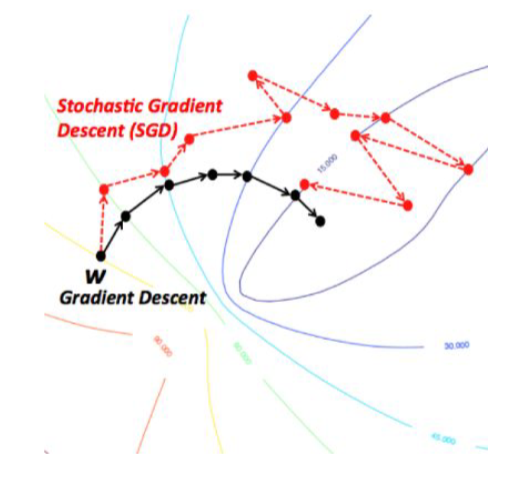
\includegraphics[width=0.35\linewidth]{SGD.png}
    \caption{Stochastic Gradient Descent}
    \label{fig:enter-label}
\end{figure}

\begin{itemize}
    \item For each iteration, evaluate a training sample from the dataset taken at random.
    \item Computing the gradient takes less time, but... may not actually be faster...
    \item Optimization path that looks rather erratic.
    \item SGD allows you to do more of a global search for an optimum, often resulting in a better set of weights for your model.
    \item Gradient Descent (GD) on the entire training data!
\end{itemize}

\begin{definition}
    \textbf{Stochastic Gradient Descent:} an optimization algorithm used to iteratively (\textbf{one at a time}) update the parameters of a model by computing the gradient of the loss function using a \textbf{randomly selected subset of the training data} in each iteration.
\end{definition}

\noindent\textbf{Mini-Batch Gradient Descent}

Instead of working with one sample at a time... can apply batching...
\begin{enumerate}
    \item Use our network to make predictions for $n$ samples
    \item Compute the average loss for those $n$ samples
    \item Take a “step” to optimize the average loss of those $n$ samples
\end{enumerate}

\begin{theorem}
    Set \textbf{batch size} close to \textbf{GPU memory} to use as much memory as possible!
\end{theorem}

\noindent\textbf{Batch size:} Number of training examples used per optimization “step”. \\
\noindent\textbf{Iteration:} One step - The parameters are updated once per iteration. \\
\textbf{Epoch:} Number of times all the training data is used once to update the parameters. \\
Suppose there are 1000 samples in the training data, if we set the batch size to 10, then 1 epoch will contain 100 iterations.

\begin{definition}
    \textbf{Mini-Batch Gradient Descent:} an optimization algorithm used to update the parameters of a model by computing the gradient of the loss function using a small subset (mini-batch) of the training data in each iteration, striking a \textbf{balance between the efficiency of Stochastic Gradient Descent (SGD) and the stability of Batch Gradient Descent}.
\end{definition}

\begin{warning}
    What happens when the \textbf{batch size is ineffective}?
    \begin{itemize}
        \item Too small:
        \begin{itemize}
            \item We optimize a (possibly very) different function loss at each iteration
            \item Noisy
        \end{itemize}
        \item Too large:
        \begin{itemize}
            \item Expensive
            \item Average loss might now change very much as batch size grows
            \item The true gradient is not always the best gradient for optimization; some
amount of noise in your gradients can help training (converge faster), so
larger batch size is not always better.
        \end{itemize}
    \end{itemize}
\end{warning}

A deep neural network has millions or billions of parameters.
Real gradient descent of a deep network is optimization in millions
of dimensions!
Most points of zero gradients are saddle points.
Plateaus are a problem but can be addressed using specialized
variants on gradient descent.\\

\noindent\textbf{Stochastic Gradient Descent (SGD) with Momentum}
\begin{figure}[h!t]
    \centering
    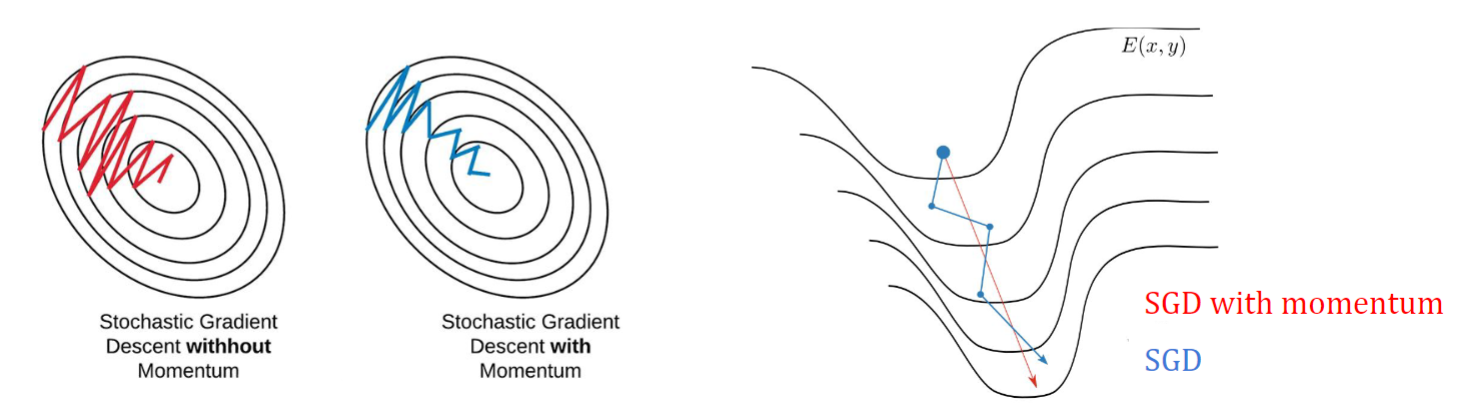
\includegraphics[width=0.7\linewidth]{SGDWM.png}
    \caption{SGD with Momentum}
    \label{fig:enter-label}
\end{figure}
\begin{definition}
    \textbf{Ravines:}  areas where the surface curves much more steeply in one dimension than in
another, common around local optima.
\end{definition}

\begin{itemize}
    \item SGD has trouble navigating ravines → it oscillates across the slopes of the ravine.
    \item Momentum helps accelerate SGD in the relevant direction and dampens oscillations.
    \item The momentum term increases for dimensions whose gradients point in the same directions and reduces updates for dimensions whose gradients change directions
    \item Analogy → we push a ball down a hill. The ball accumulates momentum as it rolls downhill, becoming faster and faster on the way until it reaches its terminal velocity

\end{itemize}

\begin{definition}
    \textbf{Stochastic Gradient Descent with Momentum:} an optimization algorithm used to iteratively update the parameters of a model by incorporating a moving average of past gradients. This momentum term helps accelerate the convergence process by reducing oscillations and smoothing out the optimization path, leading to faster and more stable convergence.
\end{definition}


\[v_{t+1} = \mu v_{t} - \alpha \nabla J(\theta_t)\]


\[\theta_{t+1} = \theta_t + v_{t+1}\]



Where:
\begin{itemize}
  \item $v_{t+1}$: Updated velocity at time step $t+1$
  \item $\mu$: Momentum coefficient (typically between 0 and 1)
  \item $v_{t}$: Velocity at time step $t$
  \item $\alpha$: Learning rate
  \item $\nabla J(\theta_t)$: Gradient of the cost (loss) function $J$ with respect to the parameters $\theta$ at time step $t$
  \item $\theta_{t+1}$: Updated parameters at time step $t+1$
  \item $\theta_t$: Parameters at time step $t$
\end{itemize}


\noindent\textbf{Adaptive Moment Estimation (Adam)}

\begin{figure}[h!t]
    \centering
    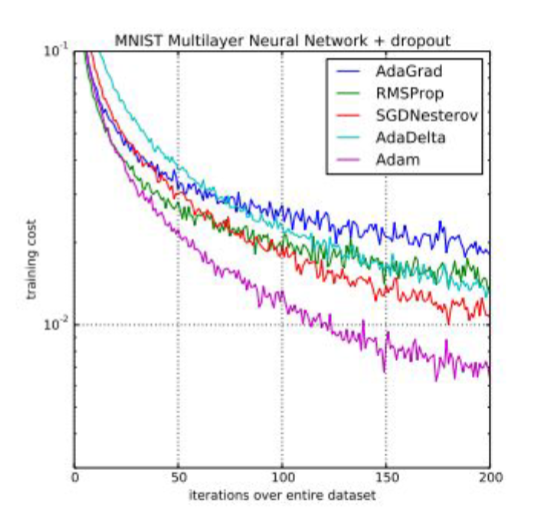
\includegraphics[width=0.4\linewidth]{optimizers.png}
    \caption{Optimizers relative to each other in terms of training cost over iterations}
    \label{fig:enter-label}
\end{figure}

\begin{definition}
    \textbf{Adaptive Moment Estimation:} a popular optimization algorithm used for tuning the parameters of a model during training. It combines concepts from both Adaptive Gradient Algorithm (AdaGrad) and Root Mean Square Propagation (RMSProp) to adaptively adjust learning rates for each parameter. This helps achieve efficient and stable convergence by individually adapting the learning rates while also incorporating momentum-based updates.
\end{definition}

\begin{itemize}
    \item Adaptive learning rates → each weight has its own rate
    \item Incorporates momentum and adaptive learning rate:
    \begin{itemize}
        \item rapid convergence
        \item requires minimal tuning
        \item commonly used optimizer
    \end{itemize}
\end{itemize}

\begin{figure}[h!t]
    \centering
    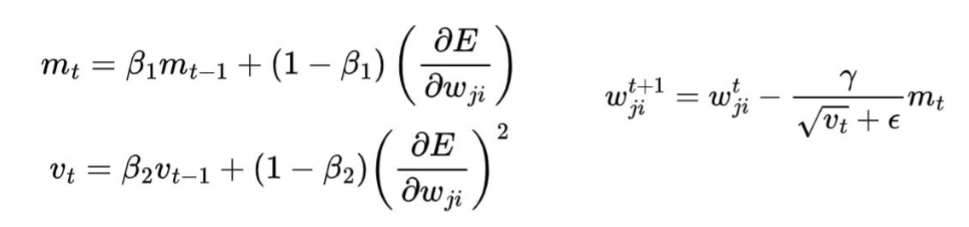
\includegraphics[width=0.4\linewidth]{adam.png}
    \caption{Adam Optimizer Equations}
    \label{fig:enter-label}
\end{figure}

\begin{idea}
    \textbf{Optimizer Summary:}\\

    1. \textbf{SGD (Stochastic Gradient Descent)}:
   \begin{itemize}
       \item \textbf{Use when:} Training on large datasets with limited computational resources.
       \item \textbf{Scenario:} Updates model parameters using the gradient of a single randomly selected data point.
       \item \textbf{Pros:} Faster updates, can escape local minima, suitable for online learning.
       \item \textbf{Cons:} Noisy updates, slower convergence on some problems.
   \end{itemize}

2. \textbf{SGD with Momentum}:
   \begin{itemize}
       \item \textbf{Use when:} Training needs faster convergence and better handling of noisy gradients.
       \item \textbf{Scenario:} Incorporates a moving average of past gradients to accelerate convergence.
       \item \textbf{Pros:} Faster convergence, reduced oscillations, better handling of noisy data.
       \item \textbf{Cons:} May overshoot in some cases.
   \end{itemize}

3. \textbf{Adam (Adaptive Moment Estimation)}:
   \begin{itemize}
       \item \textbf{Use when:} Training deep neural networks with diverse architectures.
       \item \textbf{Scenario:} Combines adaptive learning rates for each parameter and momentum-like behavior.
       \item \textbf{Pros:} Fast convergence, adaptive learning rates, well-suited for complex models.
       \item \textbf{Cons:} Can require tuning, memory-intensive.
   \end{itemize}

4. \textbf{Mini Batch Gradient Descent}:
   \begin{itemize}
       \item \textbf{Use when:} Training on medium to large datasets efficiently.
       \item \textbf{Scenario:} Computes gradient on a small subset (mini-batch) of data.
       \item \textbf{Pros:} Faster convergence than pure SGD, benefits from vectorized operations.
       \item \textbf{Cons:} Batch size selection matters, noise in updates, needs more memory.
   \end{itemize}
\end{idea}


\section{Learning Rate}

The learning rate determines the \textbf{size of the step} that an optimizer takes during each iteration. Larger step size means a bigger change in the parameters (weights) in each iteration.

\begin{figure}[h!t]
    \centering
    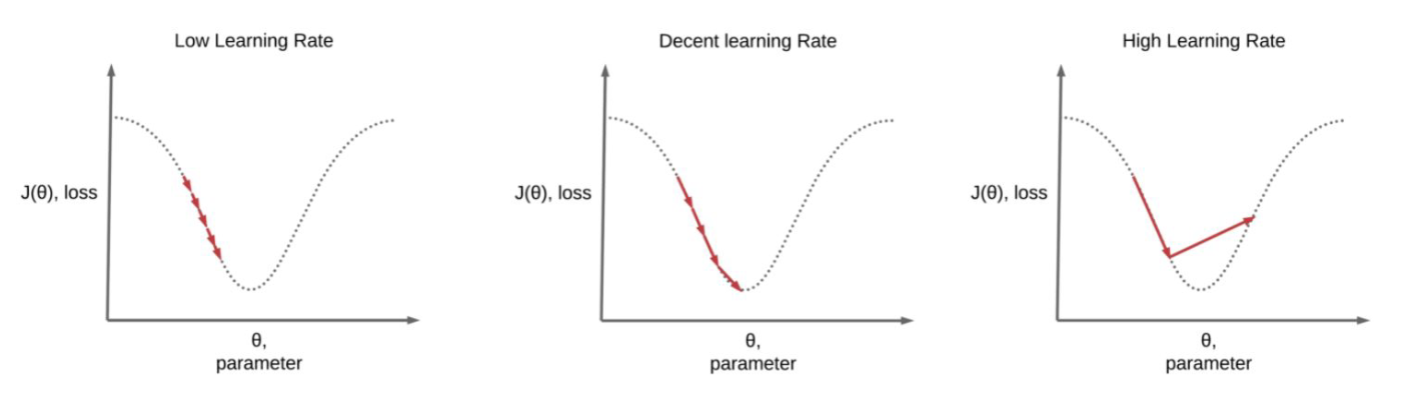
\includegraphics[width=0.8\linewidth]{learningrate.png}
    \caption{Learning Rate Size}
    \label{fig:enter-label}
\end{figure}

\begin{warning}
    What happens when the \textbf{learning rate size is ineffective}?
    \begin{itemize}
        \item Too small:
        \begin{itemize}
            \item Very small parameter change
            \item Longer training time
        \end{itemize}
        \item Too large:
        \begin{itemize}
            \item Noisy
            \item Detrimental to training
        \end{itemize}
    \end{itemize}
\end{warning}

\begin{figure}[h!t]
    \centering
    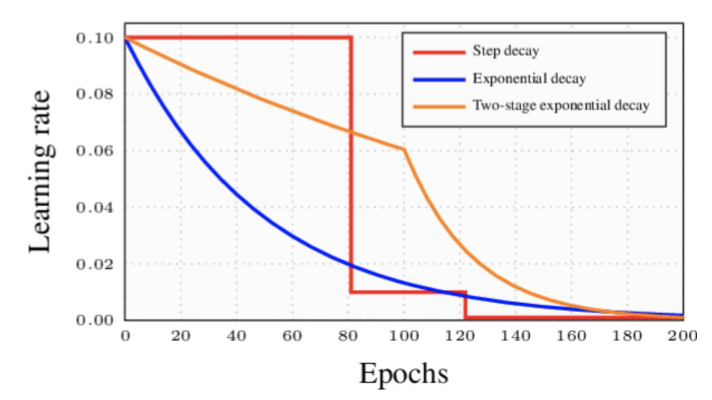
\includegraphics[width=0.5\linewidth]{learningrateoverepochs.png}
    \caption{How learning rate changes over epochs}
    \label{fig:enter-label}
\end{figure}

\textbf{The appropriate learning rate depends on:}
\begin{itemize}
    \item The learning problem
    \item The optimizer
    \item The batch size
    \begin{itemize}
        \item \textbf{Large batch}: larger learning rates
        \item \textbf{Small batch}: smaller learning rates
    \end{itemize}
    \item The stage of training
    \begin{itemize}
        \item Reduces as training progresses
    \end{itemize}
\end{itemize}

\section{Normalization}

\begin{definition}
   \textbf{Normalization:} refers to the process of \textbf{scaling and shifting} input data or intermediate activations to ensure that they have a \textbf{consistent and suitable range}. This aids in improving the stability and convergence of training by mitigating issues related to varying magnitudes of data across features or layers.
\end{definition}
We always normalize the inputs to prevent the model from paying attention to the features with larger range.

\[X_i = \frac{X_i - \mu_i}{\sigma_i}\]

Where:
\begin{itemize}
  \item $X_i$ is the original value of the $i$th element in the data vector.
  \item $\mu_i$ is the mean (average) of all $i$th elements across a batch of data.
  \item $\sigma_i$ is the standard deviation of all $i$th elements across the same batch of data.
\end{itemize}

\begin{figure}[h!t]
    \centering
    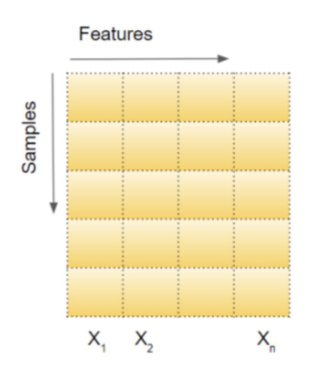
\includegraphics[width=0.3\linewidth]{normalization.png}
    \caption{Normalization}
    \label{fig:enter-label}
\end{figure}
\begin{itemize}
    \item However, this only normalizes data for the first layer. How do we normalize activations of each layer for the next layer?
\end{itemize}

\noindent\textbf{Batch Normalization}

\begin{definition}
    \textbf{Batch Normalization:} a technique used to normalize the activations of a layer by adjusting them to have zero mean and unit variance across a mini-batch of training examples. This improves training stability, speeds up convergence, and enables higher learning rates by reducing the internal covariate shift problem.
\end{definition}

\begin{theorem}
    \textbf{Internal Covariate Shift Problem:}  the change in the distribution of the input to a given layer during training. As the network learns and its parameters get updated, the distribution of activations in each layer may shift, making the optimization process more difficult. This can slow down training and require the use of lower learning rates to prevent the network from diverging or getting stuck.
\end{theorem}

Batch normalization essentially combats the internal covariate shift problem by normalizing the inputs of each layer within a mini-batch during training.

\begin{figure}[h!t]
    \centering
    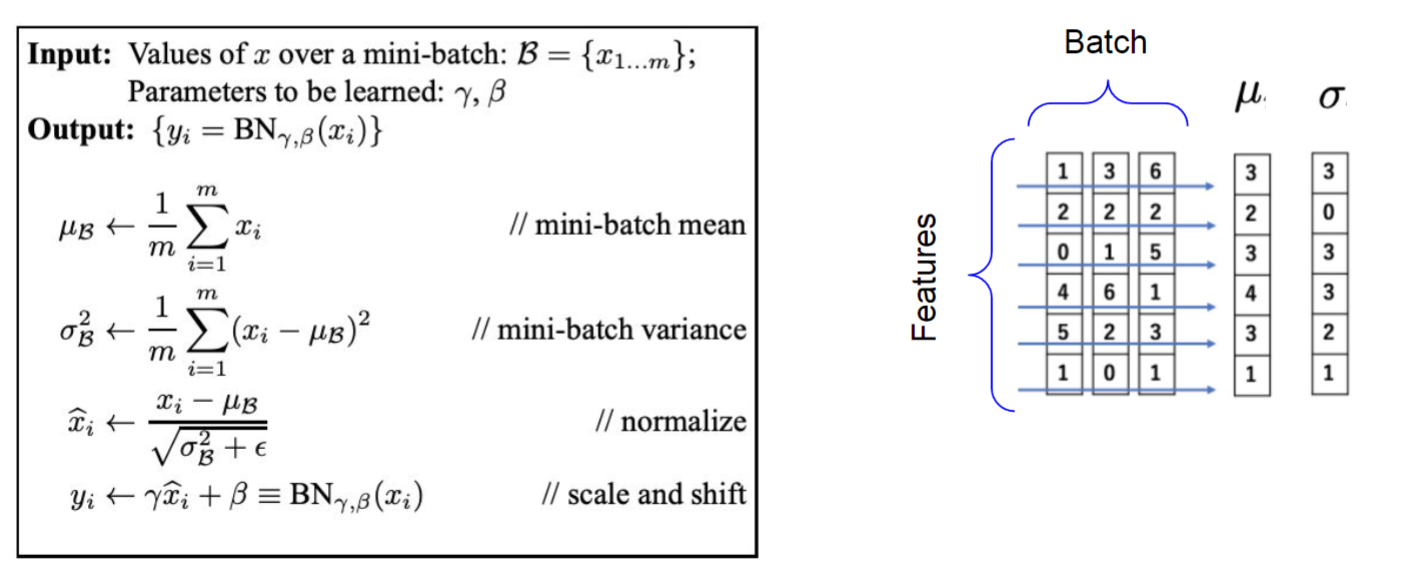
\includegraphics[width=0.75\linewidth]{batchnormalization.png}
    \caption{Batch Normalization}
    \label{fig:enter-label}
\end{figure}

\begin{definition}
    \textbf{Inference Time:} refers to the phase when a trained machine learning model is applied to new, unseen data to make predictions or produce outputs based on the knowledge it gained during its training phase.
\end{definition}

Batch Normalization primarily affects the \textbf{training phase} of a neural network, and its operation during inference time differs slightly from its behavior during training. During training, Batch Normalization computes the mean and standard deviation of each feature within a mini-batch of data, normalizes the features, and then scales and shifts them based on learnable parameters. These normalization statistics can change from one batch to another, helping with faster convergence and better generalization.\\

However, during inference time, the model processes individual examples or small batches of examples one at a time, rather than in the larger training batches. This raises the question of how to handle the normalization statistics, as there is no longer a batch of data to compute them from.\\

A way to solve this issue is \textbf{Moving Average}. 

\begin{definition}
    \textbf{Moving Average:} addresses the challenge of Batch Normalization during inference by maintaining running statistics, including the\textbf{ mean} and \textbf{standard deviation} of features, over the course of training. These running statistics are computed by \textbf{aggregating the statistics from all training batches}. During inference, these \textbf{accumulated statistics are used to normalize the input features}, providing a consistent behavior that aligns with the model's learned behavior during training. This method helps ensure that the benefits of Batch Normalization are retained when making predictions on new data while avoiding the need to compute statistics on small inference batches.
\end{definition}

\begin{figure}[h!t]
    \centering
    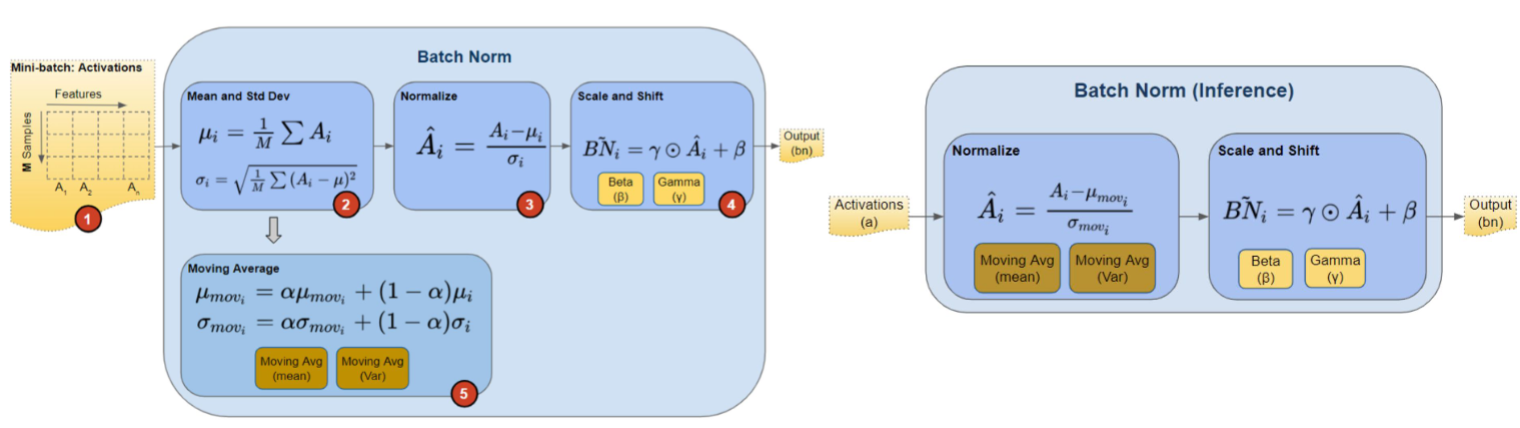
\includegraphics[width=1\linewidth]{batchnormalizationinference.png}
    \caption{Inference Time}
    \label{fig:enter-label}
\end{figure}

\noindent\textbf{Pros:}
\begin{itemize}
\item Higher learning rate $\rightarrow$ speeding up the training
\item Regularizes the model
\item Less sensitivity to initialization
\end{itemize}
\textbf{Cons:}
\begin{itemize}
\item Depends on batch size $\rightarrow$ No effect with small batches
\item Cannot work with SGD\\
\end{itemize}

\begin{warning}
    If the batch size is 1, we cannot use batch normalization!
\end{warning}

\noindent\textbf{Layer Normalization}

\begin{definition}
    \textbf{Layer Normalization:} a technique used to normalize the activations of a layer across the entire batch, focusing on the mean and standard deviation of each feature independently. This helps stabilize training, improve convergence, and reduce sensitivity to weight initialization, enhancing the network's performance.
\end{definition}

\begin{figure}[h!t]
    \centering
    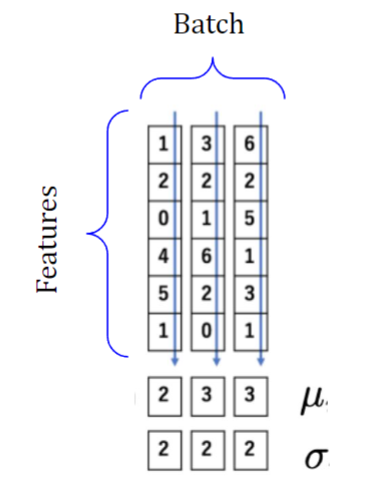
\includegraphics[width=0.25\linewidth]{layernorm.png}
    \caption{Layer Normalization}
    \label{fig:enter-label}
\end{figure}

\begin{itemize}
    \item Normalization is applied on the neuron for a single instance across all features
    \item Simpler to implement, no moving averages or parameters
    \item Not dependent on batch size
    \item Works on par with batch normalization or even better
\end{itemize}

\section{Regularization}

\begin{definition}
    \textbf{Regularization:} refers to techniques that mitigate overfitting by adding constraints or penalties to the model's training process. These techniques discourage the model from fitting noise in the training data and encourage it to learn more generalizable patterns, ultimately enhancing its ability to perform well on unseen data. Essentially, \textbf{techniques that make it hard for the model to memorize.}
\end{definition}

\textbf{Dropout}

\begin{definition}
    \textbf{Dropout:}  involves randomly \textbf{deactivating} (dropping out) \textbf{a proportion of neurons} during each training iteration. This helps prevent overfitting by encouraging the network to learn more robust and independent features, improving its generalization on new data.
\end{definition}

\begin{figure}[h!t]
    \centering
    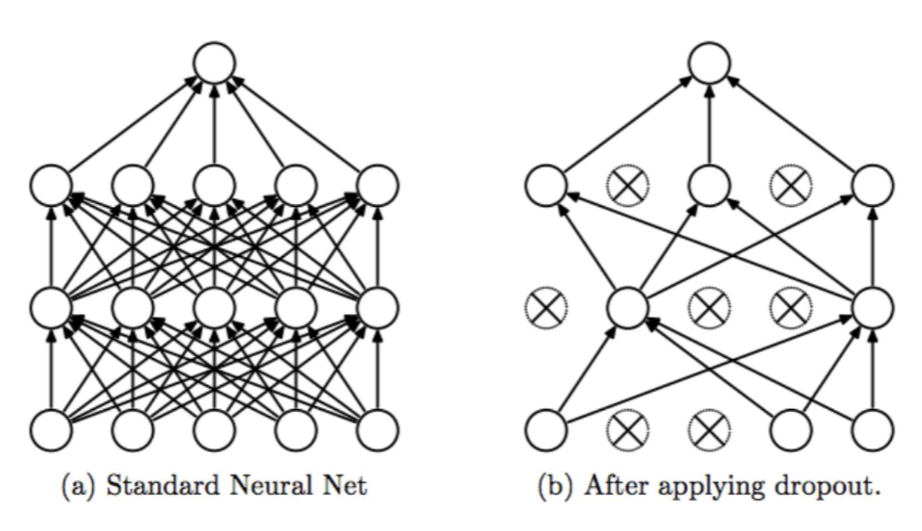
\includegraphics[width=0.5\linewidth]{dropout.png}
    \caption{Dropout}
    \label{fig:enter-label}
\end{figure}
\begin{itemize}
    \item Forces a neural network to learn more robust features by forcing to learn the \textbf{underlying distribution} of the data rather than memorizing it
    \item A very \textbf{straightforward} and \textbf{efficient} way to regularize deep models
    \item During training → Drop activations (set to 0) with probability p
    \begin{itemize}
        \item Implementation wise, neurons are muliplied by 0 to drop, and 1 to be kept
    \end{itemize}
    \item During inference → multiply weights by (1-p) to keep the same distribution
\end{itemize}

\noindent\textbf{Weight Decay (L2)}
\begin{definition}
    \textbf{Weight Decay (L2):} a technique that involves adding a \textbf{penalty term (summation of all weights of the network) to the loss function} during training. This penalty discourages the model from assigning excessively large weights to its parameters, promoting simpler and more generalizable solutions, which reduces the risk of overfitting.
\end{definition}

\begin{figure}[h!t]
    \centering
    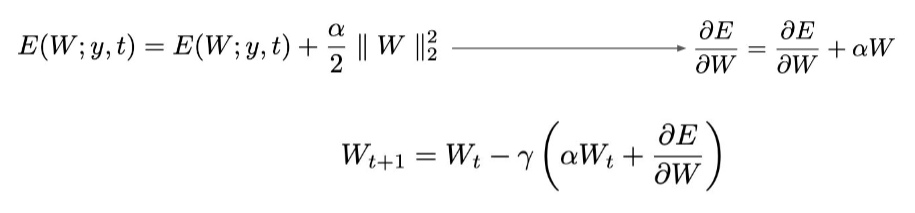
\includegraphics[width=0.75\linewidth]{weightdecay.png}
    \caption{Weight Decay}
    \label{fig:enter-label}
\end{figure}

\begin{itemize}
    \item When a model "wants" to overfit or memorize, it tends to \textbf{inflate} weights, which causes the space to be warped in a strange way, leading to memorization
    \item Prevents the weights from growing too much → Lowering variance
    \item Weight reduction is multiplicative and proportion to the scale of W
\end{itemize}

\noindent\textbf{Early Stopping with Patience}
\begin{definition}
    \textbf{Early Stopping with Patience:} refers to \textbf{monitoring} the model's performance on a validation set during training and \textbf{halting} the training process when the performance stops improving for a certain number of consecutive epochs (patience). This technique prevents overfitting by selecting a model that achieves good validation performance before it starts to degrade due to excessive training.
\end{definition}

\begin{figure}[h!t]
    \centering
    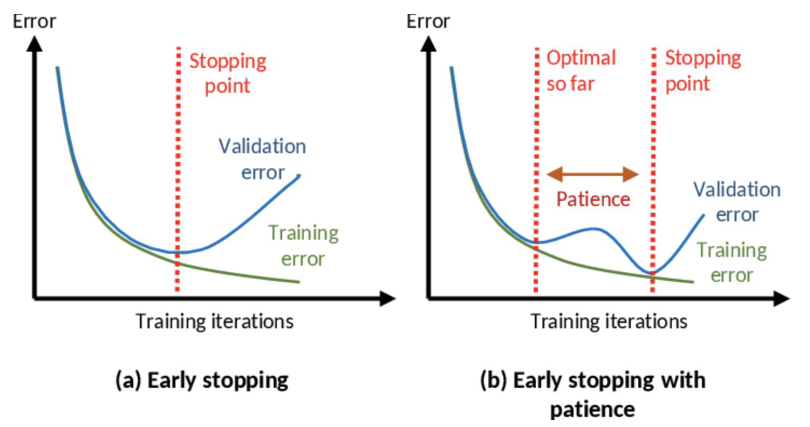
\includegraphics[width=0.75\linewidth]{earlystopping.png}
    \caption{Early Stopping with Patience}
    \label{fig:enter-label}
\end{figure}

\begin{itemize}
    \item In each training iteration observe the validation loss
    \item As soon as validation loss starts to increase, start a counter
    \item If the validation loss decreases, reset the counter
    \item Otherwise, wait for a fixed iterations (patience) and then stop the training
\end{itemize}

\section{Evaluation and Debugging}
\textbf{Debugging Tips}
\begin{itemize}
    \item Make sure your model \textbf{can overfit}
    \begin{itemize}
        \item Make sure you can get loss to decrease w.r.t training data
        \item If model cannot even learn the training data, it's not going to be able to predict validation or test data
    \end{itemize}
    \item Make sure that your network is training: i.e. loss is going down.
    \begin{itemize}
        \item Sanity check!
    \end{itemize}
    \item Ensures that you are using the right variable names, and rule out other programming bugs that are difficult to discern from architecture issues.
    \item Confusion Matrix
    \begin{itemize}
        \item True Positive (TP), False Positive (FP), True Negative (TN), False Negative (FN)
    \end{itemize}
    \item 2D Projections of Data (visualizing class clusters)
    \begin{itemize}
        \item PCA, t-SNE
    \end{itemize}
\end{itemize}

\noindent\textbf{Confusion Matrix}

\begin{definition}
    \textbf{Confusion Matrix:} tabular representation used to display the performance of a classification model. It summarizes the predicted class labels against the actual class labels, showing counts of true positive, true negative, false positive, and false negative predictions.
\end{definition}

\begin{figure}[h]
    \centering
    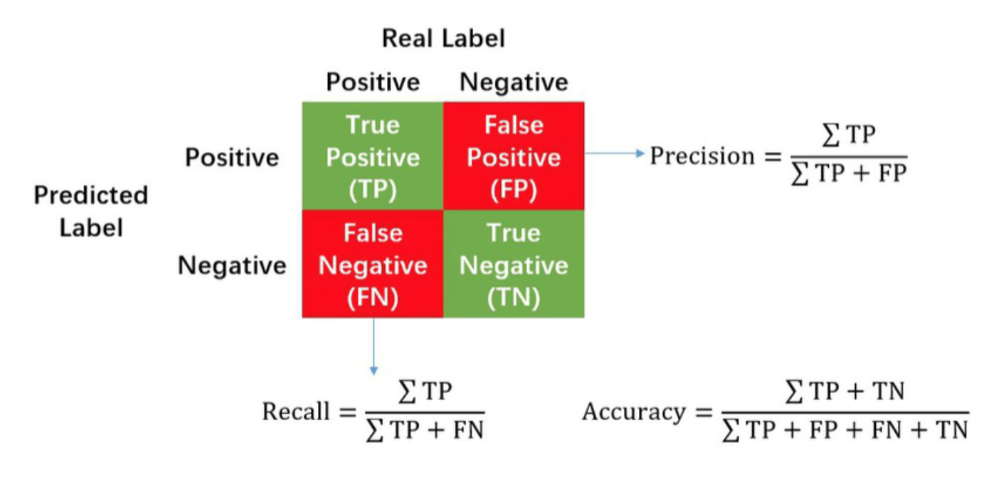
\includegraphics[width=0.7\linewidth]{confusionmatrix.png}
    \caption{Confusion Matrix}
    \label{fig:enter-label}
\end{figure}

\begin{warning}
    \textbf{Accuracy} is only valid when class distributions are equal (\textbf{balanced dataset})! \textbf{F1 Score} should be used in cases where the \textbf{dataset is unbalanced}.
\end{warning}

\begin{figure}[h!t]
    \centering
    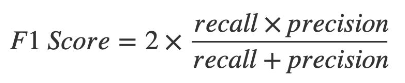
\includegraphics[width=0.45\linewidth]{f1.png}
    \caption{F1 Score}
    \label{fig:enter-label}
\end{figure}

\begin{figure}[h!t]
    \centering
    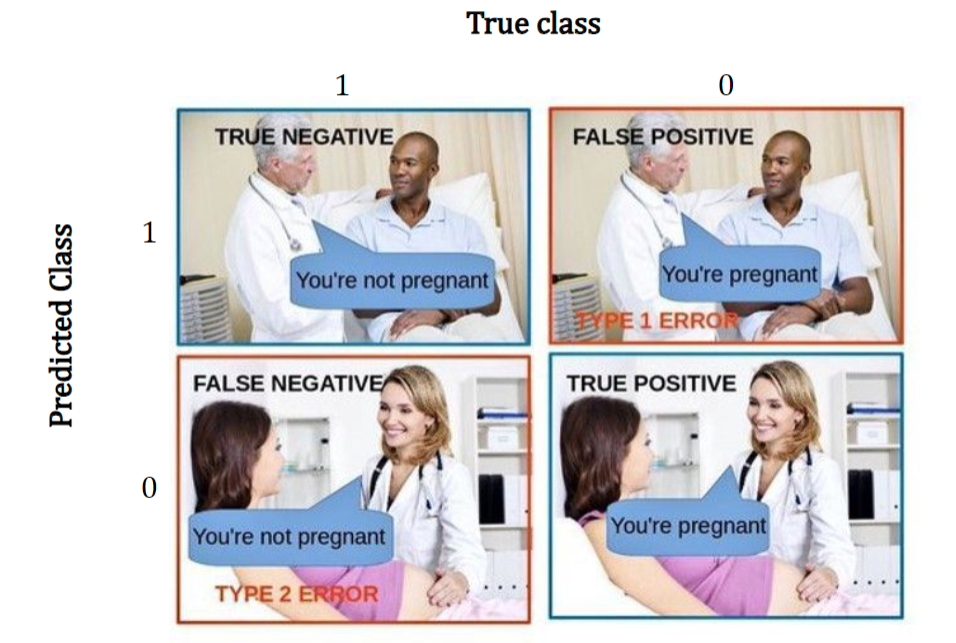
\includegraphics[width=0.5\linewidth]{ConfusionMatrixEx.png}
    \caption{Confusion Matrix Example}
    \label{fig:enter-label}
\end{figure}


\newpage

\textbf{MNIST 2D Visualization}

\begin{figure}[h!t]
    \centering
    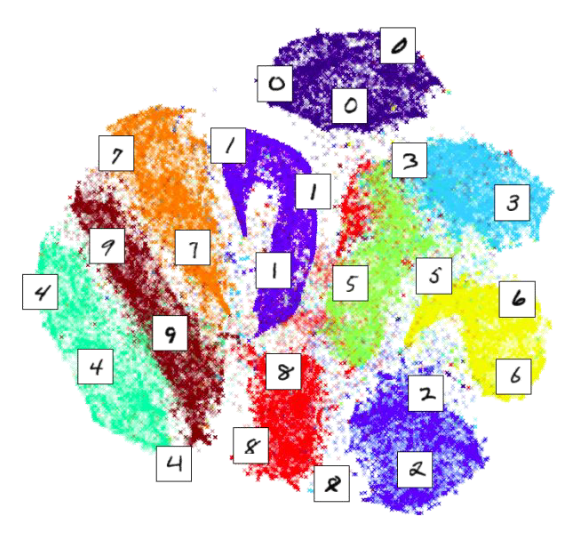
\includegraphics[width=0.4\linewidth]{2ddatavis.png}
    \caption{t-SNE for 2D projection and
visualization of data structure}
    \label{fig:enter-label}
\end{figure}

\begin{idea}
    Data that appears neatly clustered in groups by class indicates a \textbf{well-performing model}.
\end{idea}